\documentclass{article}

%links im inhaltsverzeichnis verwenden
\usepackage{hyperref}

%Damit die Überschrift vom Inhaltsverzeichnis auf Deutsch angezeigt wird
\usepackage[ngerman]{babel}

% Damit umlaute richtig angezeigt werden
\usepackage[utf8]{inputenc}

% Randabstände anpassen
\usepackage[left=2cm,right=2cm]{geometry}

% wenn man blocksatz verwenden will. Nutze \justify  oder \section{justify} für blocksatz
%\usepackage{ragged2e}

% schriftart arial verwenden
\usepackage{arial}

% package für das Einbinden von Grafiken
\usepackage{graphicx}


%farben setup für links
\hypersetup{
    colorlinks=true,
    linkcolor=black,
    filecolor=magenta,      
    urlcolor=cyan,
}



%---------------------------------- Literaturverzeichnis
\usepackage[backend=biber]{biblatex}
\addbibresource{literatur.bib}

%-------------------------------------------------------


\begin{document}

%Inhaltsverzeichnis
\newpage
\tableofcontents
\newpage

%Abbildungsverzeichnis
\newpage
\listoffigures
\newpage

%Beginn des Dokuments

\section{Einleitung}
Dieser Abschnitt führt in das Projekt ein.

\subsection{Projektumfeld}
- Kurze Vorstellung des Ausbildungsbetriebs (Geschäftsfeld, Mitarbeiterzahl usw.) \linebreak
- Wer ist Auftraggeber/Kunde des Projekts?

\subsection{Projektziel}

\subsection{Projektbegründung}

\subsection{Projektschnittstellen}

\subsection{Projektabgrenzung}

\section{Analyse}

\section{Planung}

\section{Entwurf}

\section{Implementierung}

\section{Validierungsphase}

\section{Dokumentation}

\section{Fazit}
trhrhtrhtrh
\linebreak
\linebreak
\linebreak
\linebreak
\linebreak
\linebreak
\linebreak
\linebreak


\section{Anhang}

\subsection{Abbildungsverzeichnis}
\begin{figure}
	\centering
	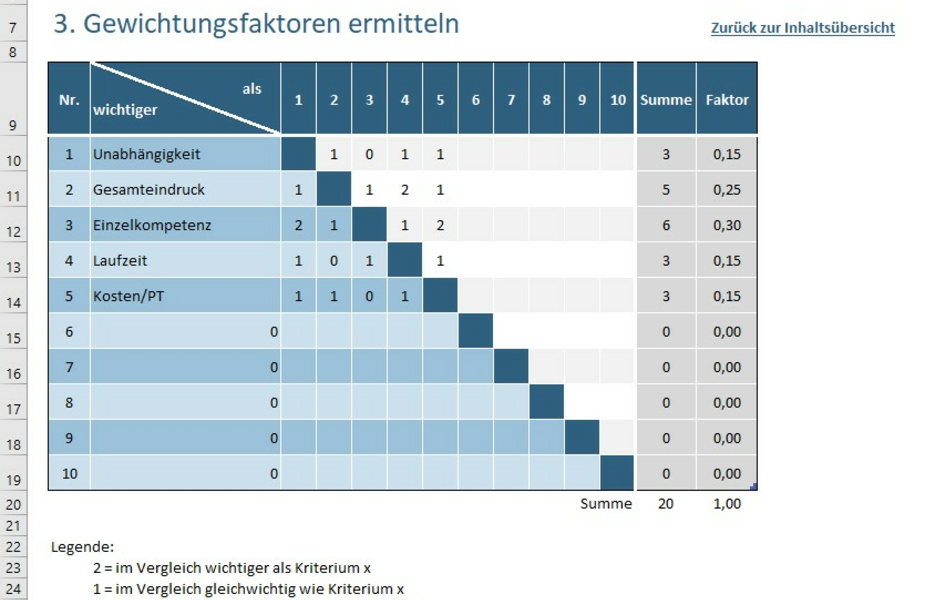
\includegraphics{nutz}
	\caption [Nutzwertanalyse]{Nutzwertanalyse}
	\label{fig:nutz}
\end{figure}

\subsection{Literaturverzeichnis}
Die mathematischen Beispiele stammen aus \autocite{Graham1995}.

Weitere Verweise: \parencite{Graham1995} oder \textcite{Thomas2008} oder sogar
\citetitle{Graham1995}.

\autocite[56]{Thomas2008}

\autocite[Siehe][45-48]{Graham1995}

Gemeinsam \autocite{Graham1995,Thomas2008}

\printbibliography

\end{document}


